
\chapter{Conclusions and Future Work} % Main chapter title

\label{Chapter6} % For referencing the chapter elsewhere, use \ref{Chapter1} 

\lhead{Chapter 6. \emph{Conclusions and Future Work}} % This is for the header on each page - perhaps a shortened title

\section{Impact	on	Society	and	the	environment}

	The environmental impact of this work is at best benign. The semiconductor industry faces a crisis because it relies on rare metals and does not take proper steps to ensure either their safe procurement or disposal. The conditions by which electronic devices are often recycled (when they are recycled) in large dumps and ludicrously unsafe working conditions in third world countries are well known. 
	
	I'm forced to wonder whether executives at TI and ST are mulling these problems over as they increasingly push their sensors and other embedded development products with the tag-line "Internet of Things". The IoT means more embedded microprocessors and sensors in increasingly cheap and disposable products, only exacerbating the unsustainable conditions that already exist. It may ultimately be a non-physical force that breaks Moore's Law. I don't believe the industry takes enough responsibility for these issues.
	
	With that said, I do believe that microelectronics represent a generally unacknowledged and misunderstood high form of art and craftsmanship. I believe that technology can empower people and have a significant positive impact on our quality of life. I also believe that this opportunity is largely squandered because technological innovation is being left largely to amoral corporate interests and should have more governmental oversight but that's another issue. I believe that transportation on this planet is set to undergo a massive reformulation as fossil fuels become increasingly problematic and alternative sources are only partially able to fill up the supply gap. Many people have already pointed out that the expansion of the middle class in India and China cannot realistically include a one-car-per-family lifestyle (see Figure \ref{f:jam}\cite{beij_traffic}). The amount of cars in the United States has already proven to be unscalable and the result of car culture on the urban landscape and social well-being to be generally bleak and negative. And the US is relatively sparsely populated compared to these emerging markets.
	
	The solution cannot be that smart cars will provide every citizen of this world with a private chauffeur. I hope that self-driving vehicles can be used to create a vastly superior system of public transportation than is currently feasible. I believe in making private ownership of vehicles illegal, or at least inverting the ratio of car lines to bus lanes in major cities. While this seems completely preposterous today, I think that a fleet of smart public transit operating on roads where human drivers are outlawed (but with heavy provisions made for pedestrian and bike traffic) will be the only way to efficiently move so many people around. (Think vast distributed network of automated Uber cars and buses that own their own traffic lanes).
	
	The domain of multicore embedded systems is in its infancy but it is crucial in realizing more sophisticated and smart robotics applications, from medical devices to automobiles to the next generation of addictive, trivial and mind-numbing commercial products. While the tools available to solve these problems are extensive, each problem is laboriously custom crafted and no generalized process exists. However, the last decade has seen much progress in defining the problem and possible paths forward. There is greater recognition that there are patterns and repetition in the individual solutions. I believe that the current state of technology is analogous to early single-core microprocessors when only assembly was available as a programming language. People eventually agreed upon less efficient but easier to program general and abstracted solutions to problems by introducing higher level programming languages. These abstractions increased the scope of a problem a single human could potentially solve with the given tool at the expense of some fine-grained efficiency losses. This work contributes a proposal to help efficiently ensure the feasibility of a multicore platform for mixed-criticality workloads.
	
\begin{figure}[h]
\centering
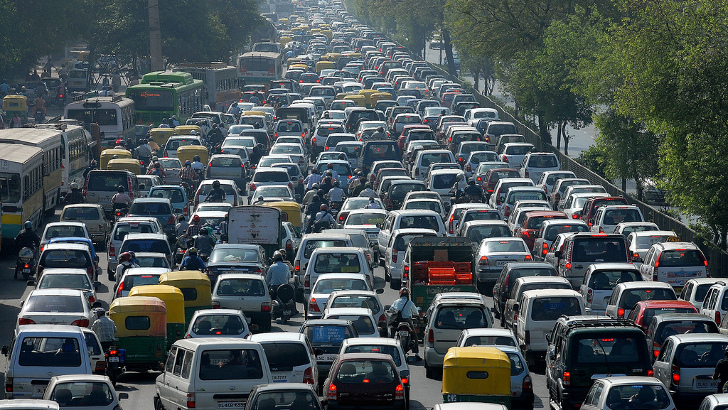
\includegraphics[width=10cm]{Figures/beijingtrafficjam.jpg}
\caption{A 12 day traffic jam occurred in Beijing in 2010.}
\label{f:jam}
\end{figure}
	
\section{Conclusions}
\label{s:conclusions}

	Heterogenous reliability architectures are a new and promising approach to deal with the variable safety requirements of mixed-criticality workloads. We have demonstrated that fingerprinting can be used to achieve dynamic core coupling and on-demand redundancy, which are themselves methods of significantly improving resource utilization when defining an application schedule and mapping to a platform. Fingerprinting represents a modest increase in logic for a multicore system while having the advantage over single core hardening techniques of being disabled (so as not to waste energy hardening non-critical tasks). Fingerprinting also provides shorter detection latencies compared to software checking on a fault tolerant core because it is not necessary to wait for the task to complete in order to verify it. By augmenting the fault tolerant core with a comparator module we remove the need for the FTC to take action until the result of a task is determined. The comparator is designed to function for up to 16 simultaneous tasks on up to 16 cores at constant cost for two way comparison and error detection. This method is not dependent on the bus topology without any special wiring. We have shown that is possible to implement fingerprinting on an FPGA platform without modifying or gaining access to the internal structure of the Nios II core. We have also demonstrated that it is possible to fingerprint a Simulink generated automotive shift logic controller requiring only modifications to the linker script and annotation of global variables in the header files. 
	
\section{Future Work}
	Several new questions arise for future research based on this prototype. Firstly, there is the possibility to recreate and extend the automated design space exploration process to include automated code generation for the platform. We can then explore the extent to which fingerprinting will affect the use of limited resources such as the data scratchpad. Secondly we can target the bus topology of our platform and replace the Altera Avalon bus with a time triggered statically scheduled bus policy. This will allow us to dramatically reduce interference in our system so that we can explore the possibility of fingerprint buffer overflow and how to mitigate it in dynamic applications with several nested tasks that all require fingerprinting.
	
	